\section{问题四模型的建立与求解}

\subsection{模型建立}

问题四要求分析园区离网运行时的能源自给状况并研究储能的最优配置。离网运行时园区与公共电网无电气连接（$P_{\mathrm{b}}(t)=P_{\mathrm{s}}(t)\equiv 0$），制氢氨功率必须跟随可再生出力变化。

离网运行下，功率平衡方程为：
\begin{equation}
P_{\mathrm{w}}(t) + P_{\mathrm{pv}}(t) = P_{\mathrm{L}}(t) + P_{\mathrm{prod}}(t) + P_{\mathrm{ch}}(t) - P_{\mathrm{dis}}(t) + P_{\mathrm{cur}}(t) \label{eq:q4_bal}
\end{equation}
其中$P_{\mathrm{cur}}(t)$为弃电功率。无储能时，$P_{\mathrm{ch}}(t)=P_{\mathrm{dis}}(t)\equiv 0$，可用功率$P_{\mathrm{avail}}(t) = \max\{0,\; P_{\mathrm{w}}(t)+P_{\mathrm{pv}}(t)-P_{\mathrm{L}}(t)\}$，制氢氨功率：
\begin{equation}
P_{\mathrm{prod}}(t) = \begin{cases}
P_{\mathrm{max}}, & P_{\mathrm{avail}}(t) \ge P_{\mathrm{max}} \\
P_{\mathrm{avail}}(t), & P_{\mathrm{min}} \le P_{\mathrm{avail}}(t) < P_{\mathrm{max}} \\
0, & P_{\mathrm{avail}}(t) < P_{\mathrm{min}}
\end{cases} \label{eq:q4_prod}
\end{equation}
其中$P_{\mathrm{min}} = 0.1P_{\mathrm{max}} = 4.15$ MW。

储能设备的荷电状态（SOC）动态方程\cite{li2023ieee}为：
\begin{equation}
E(t+1) = E(t)(1-\delta) + P_{\mathrm{ch}}(t)\eta_{\mathrm{ch}} - \frac{P_{\mathrm{dis}}(t)}{\eta_{\mathrm{dis}}} \label{eq:q4_soc}
\end{equation}
其中各参数如\cref{tab:q4_storage_params}所示。约束条件包括$0 \le E(t) \le E_{\mathrm{max}}$、充放电功率限制及充放电互斥。

\begin{table}[H]
\centering
\caption{储能设备参数}
\label{tab:q4_storage_params}
\begin{tabular*}{\textwidth}{@{\extracolsep{\fill}}lc}
\toprule[1.5pt]
参数 & 取值 \\
\midrule[1pt]
自损耗率$\delta$ & 0.2\% \\
充电效率$\eta_{\mathrm{ch}}$ & 90\% \\
放电效率$\eta_{\mathrm{dis}}$ & 90\% \\
投资成本 & 1000 元/kWh \\
使用寿命 & 15 年 \\
\bottomrule[1.5pt]
\end{tabular*}
\end{table}

储能容量优化采用双层模型：外层枚举$E_{\mathrm{max}} \in [0, 200]$ MWh，目标为最小化年均吨氨成本（含储能投资折旧和运维）；内层在每种风光场景下优化逐时调度，使可再生能源利用最大、弃电最小。

\subsection{模型求解}

\textbf{离网无储能求解。}对每个场景$t=0,\ldots,23$：
\begin{enumerate}
    \item 计算可用功率$P_{\mathrm{avail}}(t) = \max\{0,\; P_{\mathrm{w}}(t)+P_{\mathrm{pv}}(t)-P_{\mathrm{L}}(t)\}$。
    \item 若$P_{\mathrm{avail}}(t) \ge 41.5$ MW，取满发$P_{\mathrm{prod}}(t)=41.5$ MW，弃电$P_{\mathrm{cur}}(t)=P_{\mathrm{avail}}(t)-41.5$。
    \item 若$4.15 \le P_{\mathrm{avail}}(t) < 41.5$ MW，按可用功率生产$P_{\mathrm{prod}}(t)=P_{\mathrm{avail}}(t)$，无弃电。
    \item 若$P_{\mathrm{avail}}(t) < 4.15$ MW，无法开机$P_{\mathrm{prod}}(t)=0$，$P_{\mathrm{avail}}(t)$全部弃掉。
\end{enumerate}
由$P_{\mathrm{prod}}(t)$累计日产量：$Q_{\mathrm{day}} = [\sum P_{\mathrm{prod}}(t)] \times 0.0723$。

以S13（风4光1）为例：白天光伏大发时段（10:00-14:00）可再生盈余50-70 MW，制氨满载41.5 MW，多余电量弃掉；夜间和傍晚盈余不足4.15 MW时停机。该场景日产量约46.2吨，弃电177.3 MWh。

\textbf{储能配置求解。}外层枚举储能容量$E_{\mathrm{max}} = 0,20,40,\ldots,200$ MWh，内层调度规则为：
\begin{enumerate}
    \item 有盈余时：先满足生产，剩余电量优先给储能充电（不超过SOC上限和充电功率限制）。
    \item 可再生不足时：若储能SOC足够，放电补充生产，使$P_{\mathrm{prod}}$达到最小开机功率以上。
\end{enumerate}
每个储能容量下计算24场景的年均吨氨成本（含储能折旧和运维），结果如\cref{fig:q15_pareto}所示。

\textbf{离网联网对比求解。}按题目要求，在相同产量下对比。对每个场景取离网产量$Q_{\mathrm{off}}$，调用问题三连续调节模型计算联网模式在同等产量下的成本，然后统计全年均值。

\textbf{结果分析。}由最大弃电场景S13的功率数据绘制离网运行功率平衡图如\cref{fig:q13_offgrid}所示。

\begin{figure}[H]
\centering
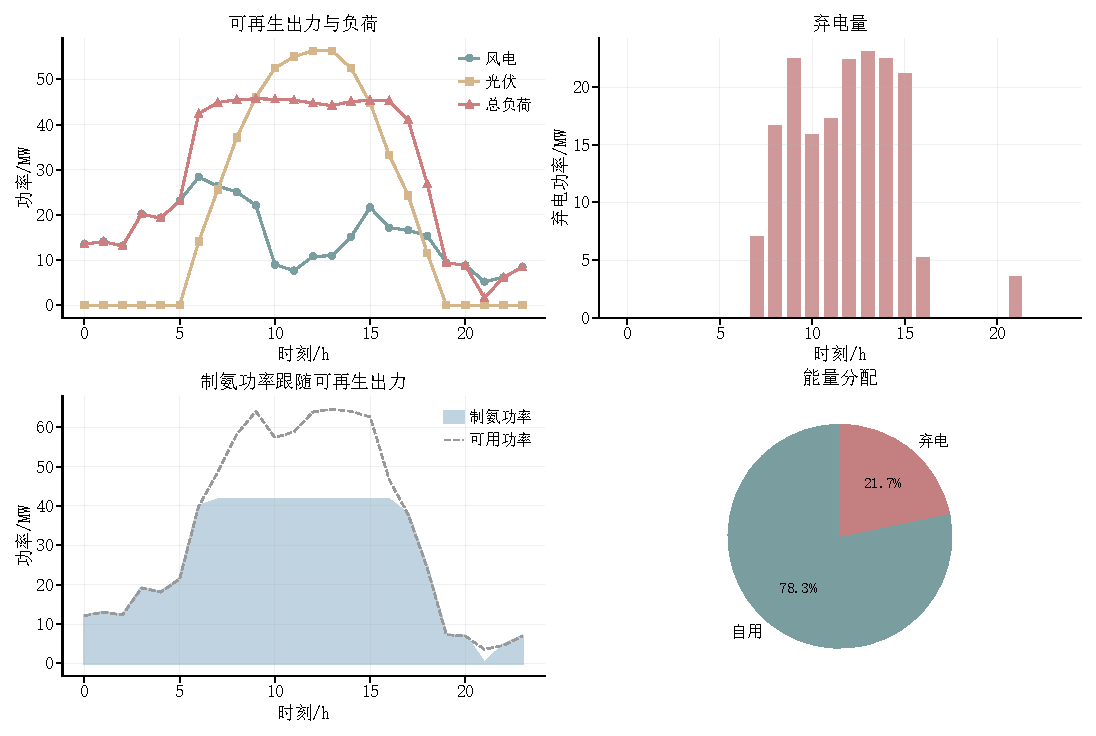
\includegraphics[width=\textwidth]{../figures/q4/fig13_offgrid_power_balance.pdf}
\caption{最大弃电场景（S13风4光1）离网运行功率平衡}
\label{fig:q13_offgrid}
\end{figure}

\cref{fig:q13_offgrid}展示了离网运行时制氨功率紧密跟随可再生出力——白天光伏大发时段制氨功率接近满载，夜间和低出力时段则下降或停机。

24场景的离网产量与弃电率分布如\cref{fig:q14_prod_curtail}所示，汇总指标见\cref{tab:q4_1}。

\begin{figure}[H]
\centering
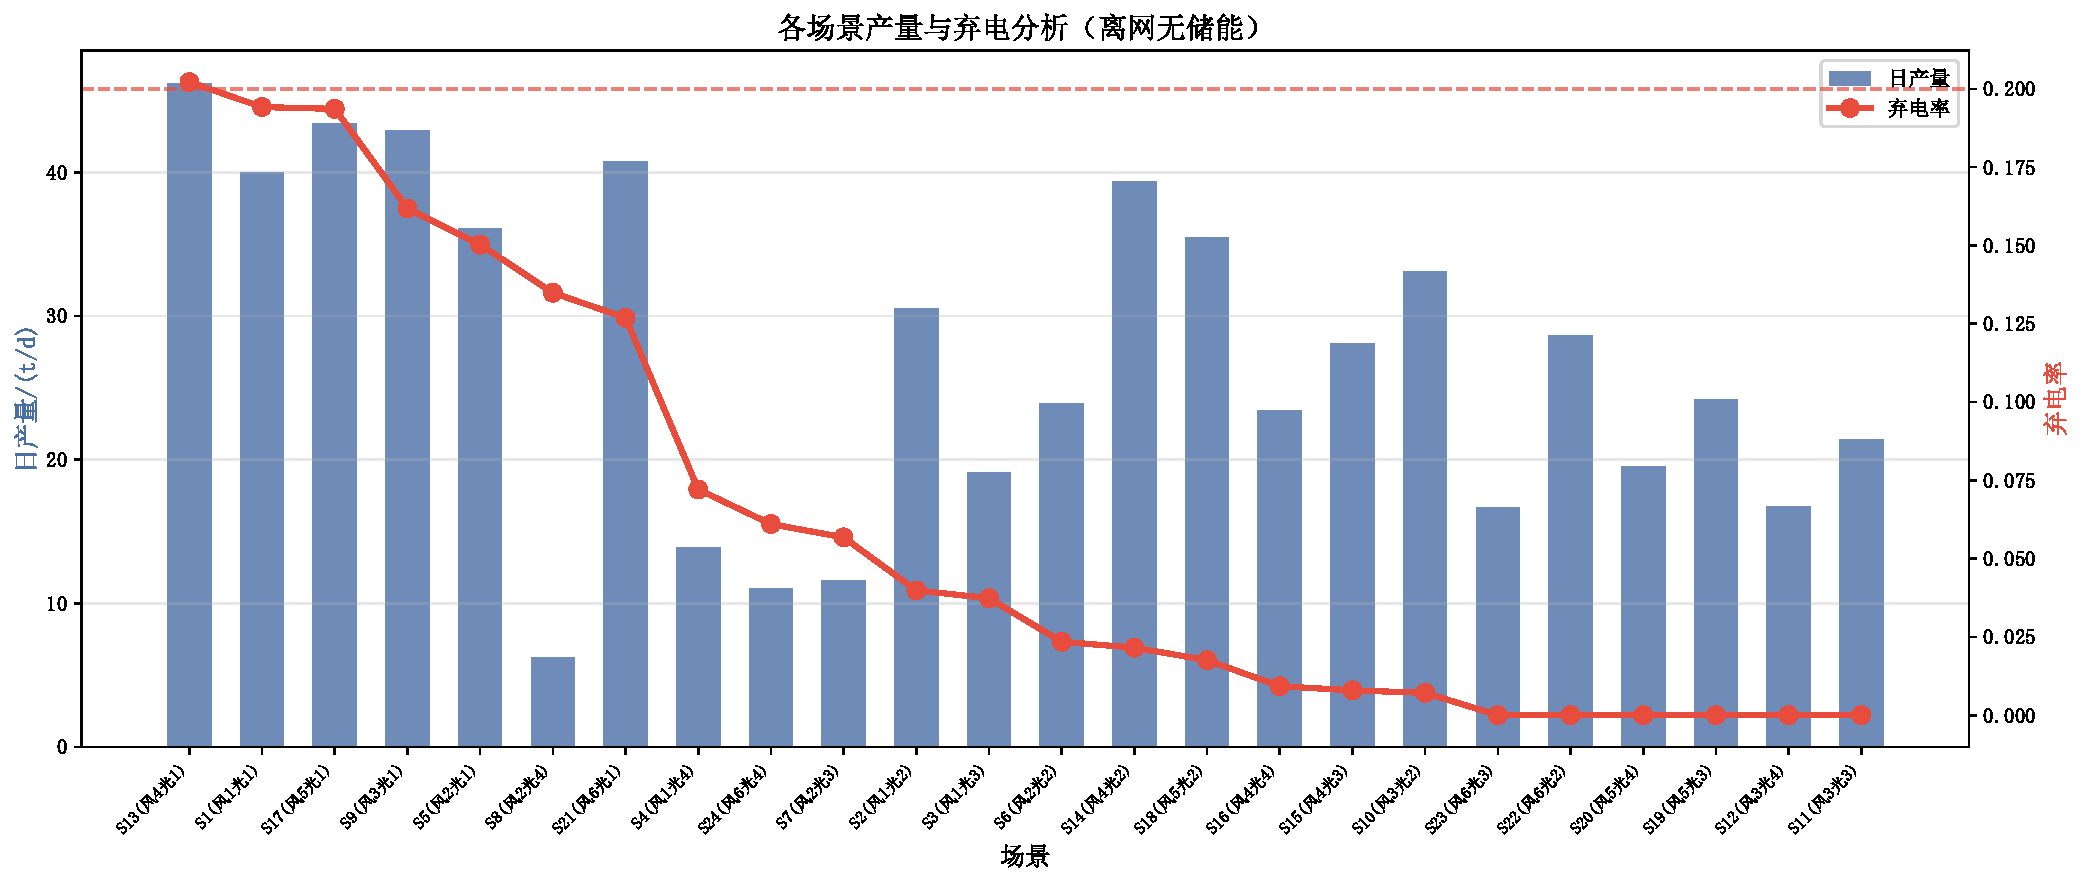
\includegraphics[width=\textwidth]{../figures/q4/fig14_production_curtail.pdf}
\caption{各场景产量与弃电率分析}
\label{fig:q14_prod_curtail}
\end{figure}

\begin{table}[H]
\centering
\caption{离网无储能运行关键指标}
\label{tab:q4_1}
\begin{tabular*}{\textwidth}{@{\extracolsep{\fill}}lc}
\toprule[1.5pt]
指标 & 数值 \\
\midrule[1pt]
全年制氨总量 & 9782 吨 \\
平均吨氨成本 & 4158 元/吨 \\
平均产能利用率 & 37.7\% \\
平均可再生利用率 & 93.7\% \\
最大弃电场景 & S13(风4光1)：177.3 MWh \\
最小产量场景 & S8(风2光4)：6.2 t/d \\
\bottomrule[1.5pt]
\end{tabular*}
\end{table}

\cref{fig:q14_prod_curtail}以场景按弃电率降序排列的方式展示了产量与弃电率的关系。总体趋势是弃电率越高的场景产量也越高，这是因为高弃电场景通常风光资源丰富（如S13风4光1），可再生出力远超制氢负荷需求，制氨功率可长时间满载运行，多余电量则被弃掉。反之，低弃电场景（如S8风2光4）风光出力偏低，可用功率经常低于最小开机阈值4.15 MW，导致产量极低但弃电也少。\cref{tab:q4_1}汇总了24场景的总体情况：全年制氨9,782吨、平均产能利用率仅37.7\%，说明离网模式下大部分时间可再生出力不足以支撑满负荷生产。

储能配置优化的Pareto曲线如\cref{fig:q15_pareto}所示。

\begin{figure}[H]
\centering
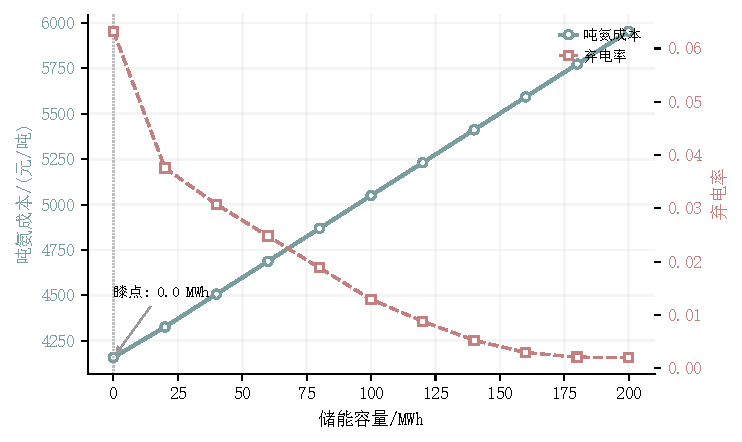
\includegraphics[width=\textwidth]{../figures/q4/fig15_pareto_storage.pdf}
\caption{储能容量优化Pareto曲线}
\label{fig:q15_pareto}
\end{figure}

\cref{fig:q15_pareto}中横轴为储能容量（0-200 MWh），左右纵轴分别为平均吨氨成本和弃电率。曲线显示随着储能容量增加，弃电率从93.7\%缓慢下降，但吨氨成本因储能投资折旧而持续上升。转折点出现在0 MWh处——配备储能后吨氨成本立即升高，而弃电率改善微乎其微（20 MWh储能仅将可再生利用率从93.7\%提升至93.9\%）。这是因为限制离网产量的根本因素是能量总量而非功率波动：即使配备储能，低风光日的总发电量也不足以满足满负荷生产需求，储能仅在少数盈余时段充放电，边际效益远低于投资成本。因此在当前储能成本（1,000元/kWh）下最优容量为0 MWh。离网与联网模式在相同产量下的对比见\cref{tab:q4_comparison}。

\begin{table}[H]
\centering
\caption{离网与联网模式综合对比（相同产量）}
\label{tab:q4_comparison}
\begin{tabular*}{\textwidth}{@{\extracolsep{\fill}}lcc}
\toprule[1.5pt]
指标 & 离网 & 联网(同等产量) \\
\midrule[1pt]
吨氨成本(元/吨) & 4158 & 3697 \\
年产量(吨) & 9782 & 9759 \\
产能利用率 & 37.7\% & 37.6\% \\
\bottomrule[1.5pt]
\end{tabular*}
\end{table}

\cref{tab:q4_comparison}表明在年产量基本持平（离网9,782吨 vs 联网9,759吨，差异仅0.2\%）的条件下，联网模式的吨氨成本为3,697元/吨，比离网模式的4,158元/吨低11.1\%。这是因为联网模式可以利用分时电价进行套利——在谷电价时段（0.3424元/kWh）从电网购电补充生产，在可再生富余时段将多余电力以0.3779元/kWh上网出售。这种灵活的双向电力交易使联网模式在相同产量下获得了显著的成本优势。
